\newpage % Rozdziały zaczynamy od nowej strony.
\section{Wprowadzenie}
\label{s_wprowadzenie}

Sztuczna skóra jest obiektem badań już od wielu lat. Naukowcy z~całego świata starają się stworzyć materiały i~układy jak najbardziej odwzorowujące skórę człowieka - zarówno pod względem wyglądu, jak i~pod względem spełnianych funkcji. Nie należy to jednak do łatwych zadań, ponieważ ludzka skóra jest bardzo skomplikowana w~budowie i~pełni wiele różnorodnych funkcji.

Skóra jest największym narządem w~ciele człowieka. Składa się ona z~trzech warstw: zewnętrznej - naskórka (odpowiada za funkcje ochronne organizmu), środkowej - skóry właściwej (umiejscowione są tam receptory, naczynia krwionośne włosowate i~gruczoły) oraz położonej najniżej - tkanki podskórnej (zapewnia ona częściowe przesuwanie się skóry nad podłożem mięśniowym oraz tworzy warstwę izolacyjną) \cite{b_book_gray}.

Jedną z~najważniejszych funkcji skóry jest funkcja ochronna. Naskórek zapewnia izolację organizmu od środowiska zewnętrznego, jest skuteczną barierą przed uszkodzeniami mechanicznymi, substancjami chemicznymi, promieniami UV, zanieczyszczeniami środowiska, niekorzystnymi dla organizmu temperaturami oraz drobnoustrojami chorobotwórczymi. 
Skóra potrafi również wytwarzać niektóre substancje pomagające w~ochronie ciała człowieka. Służą do tego gruczoły łojowe i~potowe regulujące natłuszczenie skóry i~temperaturę ciała \cite{b_unpublic_skin_1, b_book_skin_2}.
Poza tym ludzka skóra odbiera również bodźce ze~świata zewnętrznego takie jak: dotyk, ból, zimno, ciepło. Dzieje się tak, ponieważ w~skórze właściwej umiejscowione są liczne receptory, odpowiedzialne za zmysł dotyku i~czucia. Znajdują się tam również nerwy, które odpowiedzialne są za przesył bodźców do mózgu, oraz naczynia krwionośne, które dostarczają do komórek niezbędny tlen oraz substancje odżywcze. Skóra człowieka jest również elastyczna oraz sprężysta, dzięki czemu potrafi wytrzymywać duże i~gwałtowne siły jednocześnie nie odkształcając się trwale, ani nie~tracąc żadnej ze swoich właściwości. Oprócz tego skóra ludzka potrafi się także sama regenerować w~przypadku wystąpienia powierzchownych uszkodzeń \cite{b_book_skin_2, b_book_skin_3}.
%% Skin: https://www.medicalnewstoday.com/articles/320435
%% Walters: Książka Kenneth A. Walters - Dermatological and Transdermal Formulations (Drugs and the Pharmaceutical Sciences_ a Series of Textbooks and Monographs) (2002) Rozdział 1. The Structure and Function of Skin  Strony 1-39


% Gruczoły łojowe, poprzez wydzielanie łoju oraz woskowiny, stanowią barierę antybakteryjną. Zapewniają one również optymalne natłuszczenie skóry i~włosów.

%Wyjątkową właściwością skóry jest zdolność do termoregulacji. Tkanka tłuszczowa, która gromadzi się w~tkance podskórnej, jest swego rodzaju warstwą izolacyjną i~chroni organizm przed wyziębieniem. W~sytuacjach, gdy jednak organizm ochładza się - mięśnie przywłosowe kurczą się powodując uniesienie się włosów na skórze, aby mogły one stanowić dodatkową ochronę przed zimnem. 
% Natomiast przez wytwarzanie potu skóra dąży do obniżenia temperatury ciała w~momentach, kiedy organizm jest przegrzany. Dodatkowo, gruczoły potowe mają również swój udział w~regulacji gospodarki wodno-elektrolitowej organizmu.

% McGrath: Ksiazka: Griffiths C, Barker J, Bleiker T, Chalmers R, Creamer D, eds. Rook’s textbook of dermatology. 9th edn. Oxford, UK: Wiley Blackwell, (2016) Volume 1 Part 1 Foundations of Dermatology Rozdział 2. McGrath JA, Uitto J. Structure and function of the skin. strony 2.1-2.48 

% Skóra człowieka zdolna jest również do syntezy cholekalcyferolu (witaminy $D_3$) pod wpływem promieni UV. Promieniowanie to inicjuje również proces melanogenezy w~skórze. Powstała w~skutek tego procesu melanina ma za zadanie ochronę organizmu przed mutagennym działaniem promieniowania ultrafioletowego. Skóra, dzięki swojej porowatej strukturze, ma możliwość wchłaniania różnych substancji z~zewnątrz, np. leków czy korzystnych dla kondycji skóry składników zawartych w~kosmetykach. 

Skonstruowanie sztucznej powłoki, która byłaby w~stanie prawidłowo naśladować tak wiele różnych właściwości, którymi charakteryzuje się ludzka skóra jest czymś trudnym do osiągnięcia. Jest to jednak również bardzo intrygujące zadanie, dlatego też to zagadnienie jest tak często i~chętnie poruszane przez naukowców z~całego świata. 

Funkcję naskórka jest w~stanie przejąć odpowiednio dobrany materiał chroniący wnętrze sztucznej skóry przed czynnikami zewnętrznymi. Problemem okazuje się być liczba różnych czynników, które sztuczna skóra powinna blokować. Projektowane rozwiązania skupiają się głównie na ograniczeniu czynników najczęściej występujących oraz najbardziej szkodliwych dla robota. Dlatego też najczęściej zewnętrzna warstwa sztucznej skóry jest projektowana, aby była odporna mechanicznie, elastyczna i~chroniła przed zanieczyszczeniem sztucznej skóry \cite{b_article_wloch_4_wytrzymalosc, b_konf_kaczka_przekroj}.

Sztuczna skóra oprócz warstwy ochronnej skupia się przede wszystkim na części percepcyjnej, czyli czujnikach nacisku zlokalizowanych wewnątrz skóry. Ta część budowy odpowiada za podobne funkcje co warstwa skóry właściwej ludzkiej skóry.
Wykonywane pomiary dzielą się na dwie grupy - pomiary nacisku i~temperatury. Pomiary temperatury często są pomijane, ponieważ sama temperatura jest parametrem wolnozmiennym w~środowisku i~nie trzeba jej mierzyć na całej powierzchni skóry. Wykonywanie pomiarów nacisku wiąże się z~koniecznością pomiaru jego siły oraz miejsca wystąpienia. Sam pomiar nacisku może być wykonany na wiele sposobów - istnieją na rynku materiały i~czujniki o~różnej zasadzie działania (pojemnościowe, indukcyjne, rezystancyjne, optoelektryczne, piezoelektryczne oraz piezorezystywne \cite{b_article_reviev_tactile_skin}). Dobór odpowiedniego sposobu powinien być uzasadniony od sposobu eksploatacji skóry.
Odbierane pomiary są wysyłane dalej do układów obsługujących czujnik, a następnie do układu sterowania robotem. Proces ten jest analogiczny do tego, jak sygnały są przekazywane do mózgu dzięki połączeniom nerwowym w~ciele człowieka.

Najgłębsza warstwa skóry ludzkiej - tkanka podskórna nie ma aż takiego znaczenia przy budowie sztucznej skóry. Jej główna cecha - możliwość regeneracji i~tworzenia nowych komórek jest na ten moment praktycznie nie do uzyskania w~zastosowaniach robotycznych. Najbliższym odpowiednikiem regeneracji jest wymiana zużytych warstw sztucznej skóry na nowe, lecz jest to wykonywane podczas serwisowania robota. Warstwa ta, mimo okrojonych funkcji, musi być wykorzystywana, ponieważ stanowi ona bezpieczne połączenie pomiędzy obudową robota, a czujnikami i~warstwą ochronną.

Na rysunku \ref{f_porownanie_skory} widoczne jest porównanie przekroju skóry ludzkiej oraz dwóch przykładowych sztucznych skór wykonanych w~różnych technologiach.

\begin{figure}[!h]
  \begin{subfigure}[t]{0.33\linewidth}
    \centering
    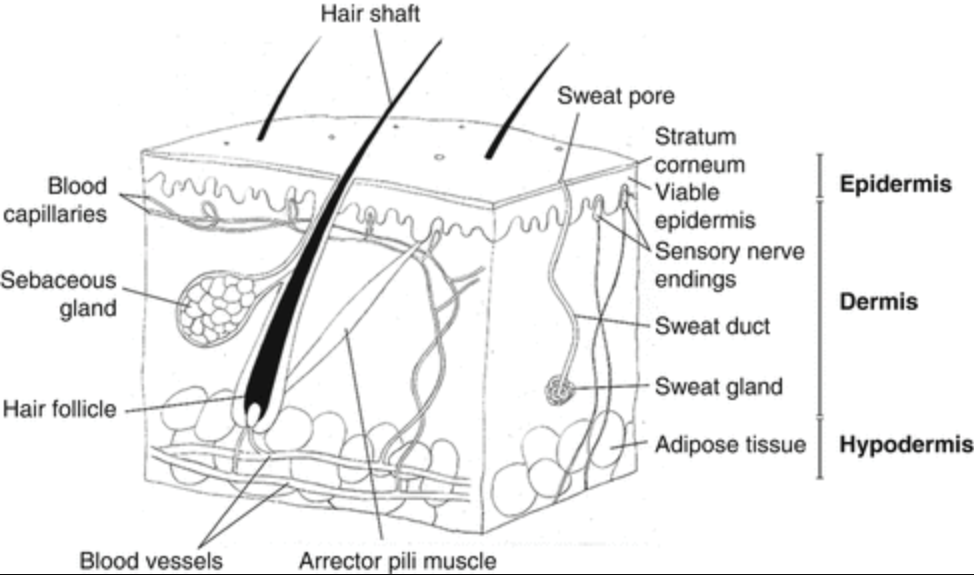
\includegraphics[width=0.95\linewidth]{img/przekroj_skory.png} 
    \caption{Skóra ludzka \cite{b_book_skin_photo}} 
    % \vspace{4ex}
  \end{subfigure}%% 
  \begin{subfigure}[t]{0.33\linewidth}
    \centering
    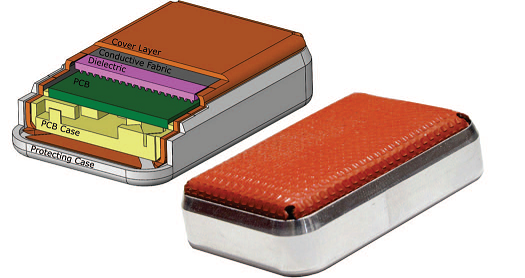
\includegraphics[width=0.95\linewidth]{img/przekroj_duck.png}
    \caption{Sztuczna skóra oparta na czujniku pojemnościowym \cite{b_konf_kaczka_przekroj}} 
    % \vspace{4ex}
  \end{subfigure}
  \begin{subfigure}[t]{0.33\linewidth}
    \centering
    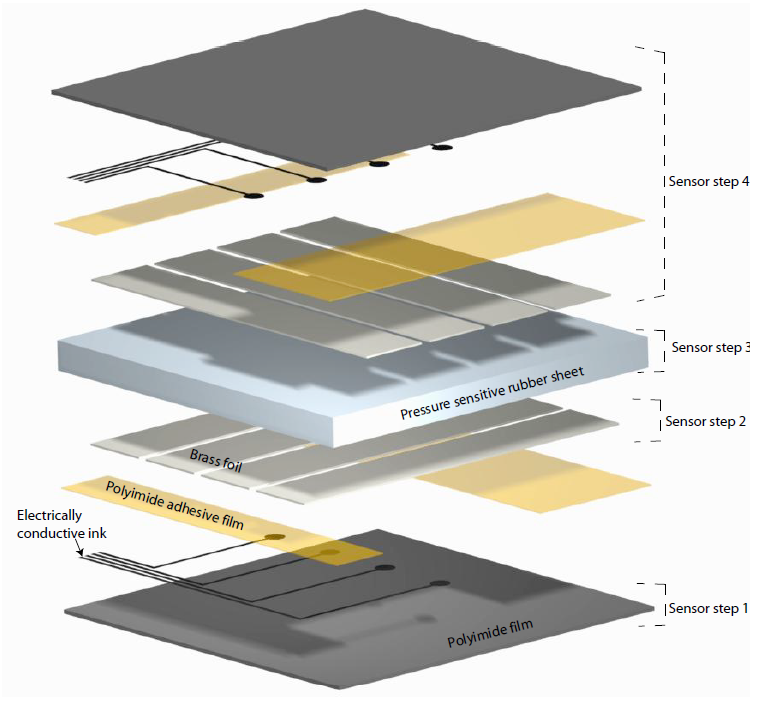
\includegraphics[width=0.95\linewidth]{img/przekroj_gietka.png}
    \caption{Sztuczna skóra oparta na warstwie o zmiennej rezystancji \cite{b_konf_gietka_przekroj}} 
    % \vspace{4ex}
  \end{subfigure}
  
  \centering
  \caption{Porównanie przekroju skóry ludzkiej i~przykładowych sztucznych skór}
  \label{f_porownanie_skory}
\end{figure}

Roboty asystujące to szczególny typ robotów przeznaczonych w~szczególności do wykonywania zleconych im zadań w~oparciu o aktualny stan siebie i~środowiska, bez ingerencji człowieka, ale we współpracy z~nim \cite{b_site_robot_definition}. Roboty asystujące z~racji na pełnione funkcje często są robotami mobilnymi posiadającymi sporą autonomiczność. Cechy te zapewniają robotowi możliwość samodzielnego poruszania się po otoczeniu oraz swobodne wykonywanie zleconych mu zadań. Swobodne poruszanie się po środowisku wymaga wykorzystywanie wielu czujników i~zabezpieczeń, aby robot nie wszedł w~kolizję ze środowiskiem. Przykładowymi kolizjami jakie mogą wystąpić są uderzenie w~ścianę bądź przedmiot lub też upadek z~krawędzi powierzchni (np. schodów). Środowisko pracy robotów asystujących jest dodatkowo utrudnione przez konieczność dzielenia jej z~istotami żywymi (ludźmi i~zwierzętami), które mogą się swobodnie poruszać lub modyfikować środowisko bez wiedzy robota.

Do pracy w~takim środowisku zachodzi potrzeba szerokiego wykorzystania wszelkiego rodzaju czujników odległości i~urządzeń mapujących otoczenie (np. LIDAR, laserowe czujniki odległości). Systemy te są szeroko wykorzystywane w~planowaniu trasy i~omijaniu przeszkód, nawet tych dynamicznie poruszających się. Systemy mapujące otoczenie są zazwyczaj umieszczane w~dolnych partiach robota, aby bardzo dobrze mapować podłoże, po którym porusza się robot. To podejście gwarantuje, że robot nie uderzy w~żaden stojący przedmiot, ani nie spadnie z~krawędzi. Problematyczna w~takim podejściu jest kwestia przedmiotów umieszczonych wyżej, które nie mają punktu podpierającego bezpośrednio pod sobą (np. blat stołu) lub są podwieszone na ścianie lub suficie. Roboty wyposażone w~czujniki na spodzie nie zawsze są w~stanie prawidłowo wykrywać tak umieszczone przeszkody.

Dodatkowo systemy wykrywające odległość nie są w~stanie bezpośrednio wykrywać wejścia robota w~kontakt z~otoczeniem. Są w~stanie wykryć tylko, że odległość robota do przeszkody jest mniejsza niż pozwala na to oprogramowanie, ale nie są w~stanie wykryć samej kolizji. W~takim wypadku (jeśli chcemy wykrywać kontakt) potrzebne nam jest rozwiązanie bazujące na sztucznej skórze. Sztuczna skóra jest zazwyczaj mocowana w~takim przypadku w~górnych partiach robota asystującego (dolna jest chroniona przez czujniki odległości), aby ochronić go przed uszkodzeniami i~pomagać mu omijać przeszkody, których nie jest w~stanie wykryć.

Robot asystujący będący już w~kontakcie z~przeszkodą może wykonać kilka akcji. Najprostszą jest zatrzymanie pracy - całkowite lub do momentu zakończenia nacisku. Jest to podejście, które poza faktem nieukończenia zadania może być niebezpieczne, ponieważ w~momencie zatrzymania robot cały czas wywiera nacisk na środowisko, potencjalnie na człowieka \cite{b_konf_collision_1}.
Innym podejściem jest wycofanie się w~miarę możliwości od elementu generującego nacisk do momentu jego zaniknięcia i~ponowne zaplanowanie nowej trasy wykonania zadania z~uwzględnieniem nowej niewykrytej wcześniej przeszkody. Podejście to zapewnia zarówno wykonanie zadania, jak i~akceptowalne oddziaływanie na środowisko.

Na rysunku \ref{f_przykladowe_roboty_uslugowe} widoczne są przykładowe roboty asystujące dostępne na rynku. Roboty przedstawione na tym rysunku przeznaczone są głównie do środowiska, gdzie muszą ściśle współpracować z~człowiekiem.

\begin{figure}[!h]
  \begin{subfigure}[t]{0.5\linewidth}
    \centering
    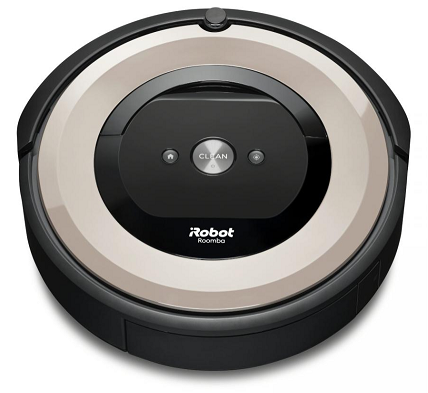
\includegraphics[width=0.7\linewidth]{img/robot_roomba.png} 
    \caption{Robot sprzątający Roomba \cite{b_site_roomba}} 
    % \vspace{4ex}
  \end{subfigure}%% 
  \begin{subfigure}[t]{0.5\linewidth}
    \centering
    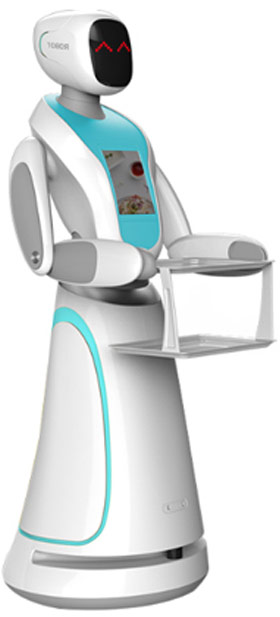
\includegraphics[width=0.4\linewidth]{img/robot_amy.jpg}
    \caption{Robot - kelner Amy \cite{b_site_Amy}} 
    % \vspace{4ex}
  \end{subfigure}
  
  \centering
  \caption{Przykładowe roboty asystujące dostępne na rynku}
  \label{f_przykladowe_roboty_uslugowe}
\end{figure}


\subsection{Motywacja}
Motywacją do wykonania prototypu sztucznej skóry była chęć rozwijania rozwiązań dotyczących sztucznej skóry, a w~szczególności wykonanie fizycznie działającej wersji i~zintegrowanie jej z~robotem. Dodatkowo chciałem poszerzyć zagadnienia związane z~problemami napotykanymi podczas budowy tego modułu robota i~testów, które trzeba wykonać na etapie planowania rozwiązania. 

Do wykonania pracy motywowała mnie również możliwość wykorzystania rozwiązania w~przyszłości w~robotach sprzedawanych powszechnie na rynku jako dodatkowa funkcja lub zabezpieczenie. Wykonany przeze mnie prototyp był testowany na robocie dostępnym na rynku, co pokazuje, że takie zastosowanie jest możliwe.

Motywacją była także chęć zintegrowania sztucznej skóry z~systemem ROS, co pozwala w~przyszłości zastosować ją na innych robotach opartych na tym systemie. 
% Zadanie to ułatwia możliwość zastosowanej zdalnej konfiguracji sterownika, którą może dokonać każdy przystosowując w~ten sposób rozwiązanie do swoich potrzeb. 
Użycie systemu ROS zwiększa także potencjalną bazę użytkowników i~ludzi, którzy mogliby dalej rozwijać wykonany przeze mnie model do innych zastosowań.

\subsection{Cel pracy}
% Prace prowadzone w~Zespole Programowania Robotów w~Zakładzie Sterowania Systemów, który funkcjonuje w~obrębie Instytutu Automatyki i~Informatyki Stosowanej na Wydziale Elektroniki i~Technik Informacyjnych na Politechnice Warszawskiej 
Prowadzone prace 
miały na celu zbudowanie sztucznej skóry wyczuwającej przykładany nacisk. Budowana skóra musiała być także jednocześnie prosta w~budowie, lekka, łatwo skalowalna, odporna mechanicznie i~możliwa do stosowania na nierównych powierzchniach.
Zbudowana sztuczna skóra miała za zadanie wspomagać robota asystującego w~poruszaniu się w~środowisku, w~szczególności chronić go przed obiektami i~uderzeniami. 
Zaproponowane rozwiązanie musiało też spełniać wymóg łatwej konfiguracji, która może być inna dla każdego zastosowania. Konfiguracja ta powinna odbywać się zdalnie, bez ingerencji w~program sterownika sztucznej skóry.

Celem pracy było również wykorzystanie zbudowanego czujnika w~praktyce poprzez umieszczenie go na robocie i~zintegrowanie go z~tym robotem. 
Integracja z~robotem miała pozwalać na zaprogramowanie robota, aby w~momencie wykrycia nacisku próbował uciec od jego źródła jeśli jest to możliwe.
% Integracja z~robotem miała pozwalać na zaprogramowanie na robocie dwóch różnych modeli zachowań:
% \begin{itemize}
%     \item wykrywanie nacisku i~próba odjechania od niego jeśli jest to możliwe
%     \item sterowanie kierunkiem ruchu robota dzięki naciskaniu na różne fragmenty skóry robota
% \end{itemize}

% Umieszczona na robocie sztuczna skóra miała za celu odbierać bodźce z~otoczenia i~przesyłać je w~przetworzonej formie do systemu sterującego robotem, aby ten podjął odpowiednie działania.

\subsection{Zakres pracy}
Praca obejmowała opracowanie prototypowego czujnika dotykowego zbudowanego jako sztuczna skóra wykrywająca siłę i~miejsce nacisku. Czujnik oparty był na folii rezystancyjnej Velostat znajdującej się pomiędzy przewodnikami elektrycznymi i~na jej właściwości do zmiany rezystancji pod wpływem przykładanego nacisku. Konstrukcja czujnika została zabezpieczona materiałem nośnym wykonanym z~gumy. Projekt ten był kontynuacją prac prowadzonych wcześniej przez Macieja Bogusza w~ramach Koła Naukowego Robotyki BIONIK \cite{b_report_otrzymane}.

Praca obejmowała przeprowadzenie badań nad wyborem optymalnego nośnika dla budowanego czujnika. Prowadzone badania obejmowały przetestowanie otrzymanego prototypu, kalibrację odczytów pomiarowych, budowę kolejnych prototypów potrzebnych do dalszych badań, jak również badanie właściwości różnych grubości użytych gum ochronnych. Badania obejmowały wykonanie charakterystyki folii Velostat w~wybranym zastosowaniu, pomiar pochłanialności energii poszczególnych grubości użytej gumy oraz rozkładanie energii wewnątrz czujnika.

Dodatkowo na potrzeby obsługi projektowanego czujnika konieczne było zaprojektowanie, wykonanie i~zaprogramowanie dedykowanego dla niego układu elektronicznego. Układ ten miał za zadanie przetwarzać dane odczytane ze sztucznej skóry i~w~przetworzonej formie przesyłać na stację roboczą - komputer z~systemem operacyjnym Linux Ubuntu do systemu sterującego robotem.

W zakres prac wchodziła także budowa sztucznej skóry zgodnie z~wynikami przeprowadzonych wcześniej badań oraz przetestowanie jej działania na fizycznie działającym robocie firmy PAL Robotics - Tiago \cite{b_site_tiago}, widocznym na rysunku \ref{f_tiago_zwykly}. Robot służący do testów działał pod kontrolą systemu ROS \cite{b_site_ROS}, więc jednym z~zadań było także dołączenie zbudowanego czujnika w~sposób kompatybilny z~wymaganiami stawianymi przez ten system.

\begin{figure}[!h]
    \centering 
    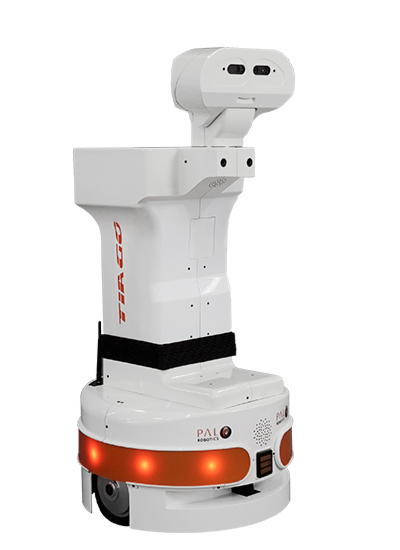
\includegraphics[width=0.5\linewidth]{img/tiago_zwykly.jpg}
    \caption{Robot Tiago \cite{b_site_tiago}}
    \label{f_tiago_zwykly}
\end{figure}

\subsection{Struktura pracy}
Niniejsza praca składa się łącznie z~ośmiu rozdziałów. W~pierwszym rozdziale zostały opisane założenia dotyczące końcowego celu jaki ta praca ma uzyskać. Opisany został też ogólny zakres prac wykonywanych podczas badań. Została także opisana motywacja jaka mną kierowała podejmując się wykonania niniejszej pracy.

Rozdział drugi opisuje przegląd istniejących na świecie rozwiązań dotyczących sztucznej skóry, jej budowy, badań nad nią i~zastosowanych rozwiązań. Zostały w~tym rozdziale opisane prace prowadzone przez innych naukowców na całym świecie i~możliwości zastosowanych przez nich podejść.

Rozdział trzeci zawiera kluczowe informacje dotyczące wykorzystanych narzędzi. Jest w~nim omówiony szczegółowo dobór zastosowanych komponentów, narzędzi i~systemów wykorzystywanych przez zbudowaną sztuczną skórę. W~tym rozdziale jest także opisana struktura systemu, do którego sztuczna skóra została dołączona i~robota, na którym była ona testowana.

Rozdział czwarty zawiera szczegółowy opis działania wybranego modelu sztucznej skóry i~podejście do zbudowania jej. W~tym rozdziale został szczegółowo przedstawiony otrzymany prototyp i~prace jakie nad nim zostały wykonane. Opisana została także budowa pozostałych warstw projektowanej przeze mnie wersji, ze szczególnym skupieniem się na sterowniku sztucznej skóry - jego elektronice i~oprogramowaniu.

% Rozdział piąty opisuje wykonane prace nad sterownikiem obsługującym projektowaną sztuczną skórę. Został opisany proces projektowania dedykowanego układu elektronicznego i~sposób obsługiwania przez niego sztucznej skóry wraz z~omówieniem wykonanego oprogramowania mikrokontrolera. Znajduje się tutaj także specyfika komunikacji układu z~komputerem nadrzędnym.

Rozdział piąty został poświęcony procesowi badań nad doborem optymalnych materiałów do budowy sztucznej skóry. Badania te prowadzone były na statycznej wersji dodatkowych mniejszych prototypów. Szczegółowo została opisana tutaj kwestia doboru odpowiedniego materiału nośnego będącego jednocześnie warstwą ochronną sztucznej skóry.

Rozdział szósty opisuje integrację sztucznej skóry z~istniejącym systemem robota. W~rozdziale tym można znaleźć szczegóły konfiguracji robota Tiago wykorzystywanego w~testach oraz proces podłączania do niego sztucznej skóry. Została także krótko opisana budowa mechaniczna zbudowanej sztucznej skóry.

Przedostatni rozdział - siódmy prezentuje wykonane testy zbudowanego czujnika, zarówno w~symulacji jak i~w~realnych warunkach. Zawarta jest w~nim weryfikacja poprawności działania w~obu tych warunkach. Przedstawiony został także drugi prototyp sztucznej skóry wraz z~powodami konieczności tworzenia kolejnej wersji czujnika.

Rozdział ósmy stanowi podsumowanie pracy. Zawarte jest w~nim podsumowanie wykonanych celów i~prac. W~rozdziale zostały także opisane wnioski jakie można wyciągnąć z~wykonanych prac.
